% VUT FIT MITAI
% MSZ 2021/2022
% Author: Vladimir Dusek
% Login: xdusek27

%%%%%%%%%%%%%%%%%%%%%%%%%%%%%%%%%%%%%%%%%%%%%%%%%%%%%%%%%%%%%%%%%%%%%%%%%%%%%%%%

% Path to figures
\graphicspath{{avs/koherence_pameti_cache/figures}}

%%%%%%%%%%%%%%%%%%%%%%%%%%%%%%%%%%%%%%%%%%%%%%%%%%%%%%%%%%%%%%%%%%%%%%%%%%%%%%%%

\chapter{AVS~--~Problém koherence pamětí cache na systémech se sdílenou pamětí, protokol MSI.}

%%%%%%%%%%%%%%%%%%%%%%%%%%%%%%%%%%%%%%%%%%%%%%%%%%%%%%%%%%%%%%%%%%%%%%%%%%%%%%%%

\section{Zdroje}

\begin{compactitem}
    \item \path{AVS-11.pdf}
    \item \path{AVS-12.pdf}
    \item \path{AVS_2019-12-02.mp4}
    \item \path{AVS_2019-12-09.mp4}
    \item \textit{Otázka je propletená s otázkou AVS 4.}
\end{compactitem}

%%%%%%%%%%%%%%%%%%%%%%%%%%%%%%%%%%%%%%%%%%%%%%%%%%%%%%%%%%%%%%%%%%%%%%%%%%%%%%%%

\section{Koherence paměti cache (CC)}

\begin{compactitem}
    \item Proč máme paměti cache? Kvůli rychlosti, přístup do paměti je příliš drahý.

    \item \textbf{Koherence pamětí cache} (CC) znamená, že pro danou adresu existuje jediná (koherentní) verze sdílených dat v jedné, několika nebo i ve všech pamětech cache. Na kopii v paměti nezáleží, ta může být zastaralá (neplatná). \begin{compactitem}
        \item Jedna adresa má stejnou hodnotu ve všech pamětích cache (nikoliv hlavní paměť)!
        \item Potřebujeme mechanismus (protokol), který toto zajišťuje.
    \end{compactitem}

    \item GPU jsou nekoherentní, synchronizace mezi tolika jádry by byla příliš náročná.

    \begin{figure}[H]
        \centering
        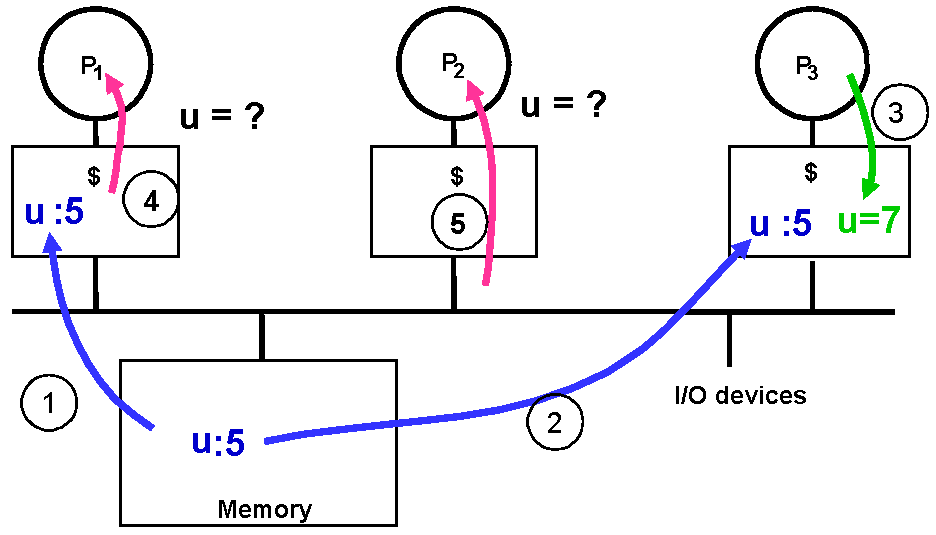
\includegraphics[width=0.75\linewidth]{koherence.pdf}
        \caption{Koherence paměti cache.}
    \end{figure}

    \item Jaké mohou být stavy bloku paměti (\textit{cache line}) v paměti cache? \begin{compactitem}
        \item \textbf{Čistý a špinavý} \begin{compactitem}
            \item Čistý -- blok se zatím pouze četl, nebylo do něho zapsáno.
            \item Špinavý -- do bloku někdo zapsal.
        \end{compactitem}
        \item \textbf{Jediný a sdílený} \begin{compactitem}
            \item Jediný -- existuje jediná kopie bloku v pamětích cache.
            \item Sdílený -- existuje několik kopií bloku v pamětích cache.
        \end{compactitem}
        \item \textbf{Platný a neplatný} \begin{compactitem}
            \item Platný -- pokud ho chce procesor číst, cache vrátí cache hit (je tam aktuální hodnota).
            \item Sdílený -- pokud ho chce procesor číst, cache vrátí cache miss (je tam neaktuální hodnota).
        \end{compactitem}

        \begin{figure}[H]
            \centering
            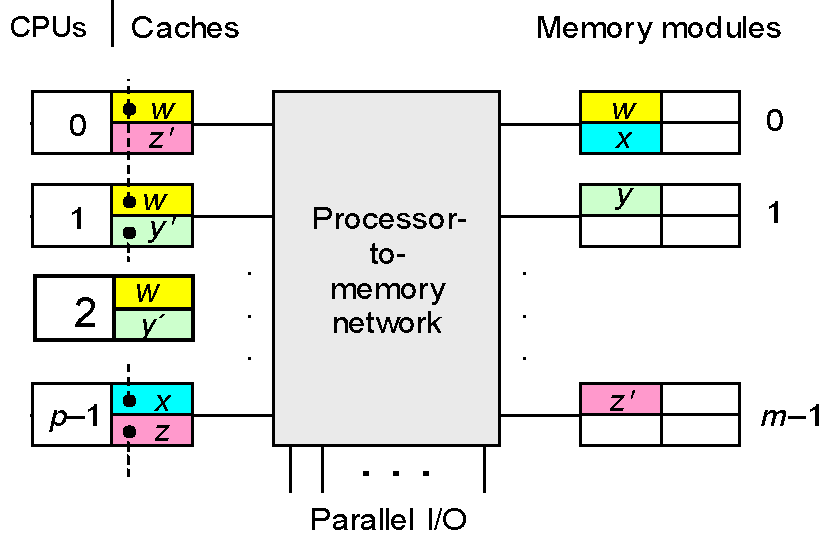
\includegraphics[width=0.75\linewidth]{typy_bloku_dat_pameti_cache.pdf}
            \caption{Každé jádro procesoru má svoji cache, memory modules je hlavní paměť. Paměťové bloky s čarou jsou modifikované. Stav bloků: $x$ je čistý, jediný a platný; $w$ je čistý, sdílený a platný; $y$ je špinavý, sdílený a platný; $z$ je špinavý, sdílený a neplatný (nekohorence).}
        \end{figure}

        \item Pro zajištění koherence pamětí cache máme 2 strategie: protokoly CC založené na monitorování komunikace a protokoly CC založené na distribuovaném adresáři.
    \end{compactitem}
\end{compactitem}

%%%%%%%%%%%%%%%%%%%%%%%%%%%%%%%%%%%%%%%%%%%%%%%%%%%%%%%%%%%%%%%%%%%%%%%%%%%%%%%%

\section{Protokoly CC založené na monitorování komunikace (naslouchání, \textit{snooping})}

\begin{compactitem}
    \item Pro systémy, které mají sběrnici a které mají broadcast. Stav bloku je připojen ke všem jeho kopiím v místních cache. Žádost s adresou bloku jde od žadatele všem (broadcast), reagují a odpovídají jen ti, kterých se to týká.

    \item Není možné modifikovat více než jednu proměnnou v jednom taktu!

    \item Většinou používají UMA systémy.

    \begin{figure}[H]
        \centering
        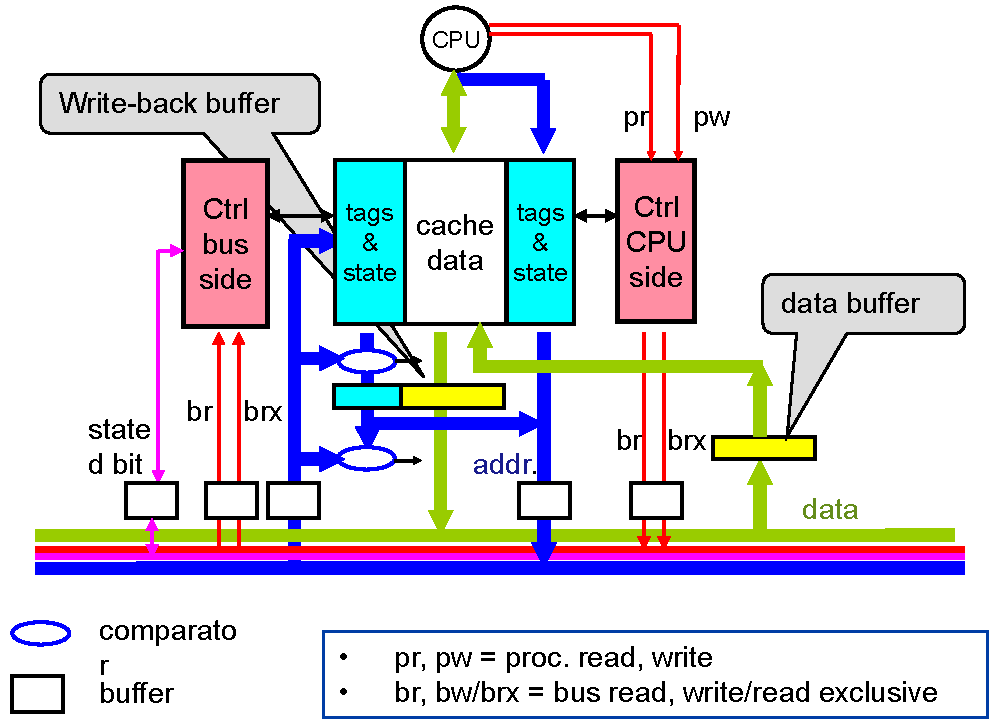
\includegraphics[width=0.9\linewidth]{radic_cache_s_naslouchanim.pdf}
        \caption{Řadič paměti cache s nasloucháním.}
    \end{figure}

    \item Aktualizace paměti -- procesor zapíše do cache, kdy data zapsat do hlavní paměti? \begin{compactitem}
        \item Při cache hit \begin{compactitem}
            \item \textbf{Write-through} -- Průpis slova do L1 a hned výš.
            \item \textbf{Write-back} -- Zpětný zápis bloku z L1 a výš až když je to nutné (musím danou cache line vyhodit).
        \end{compactitem}

        \item Při cache miss \begin{compactitem}
            \item \textbf{Write-allocate} -- Chci aktualizovat data, ale v L1 nejsou, musíme najít místo, natáhnout data z vyšší úrovně a pak je přepsat.
            \item \textbf{Write-around} -- Chci aktualizovat data, ale v L1 nejsou, tak chodím o úroveň výš, dokud data nenajdu a přepíšu je tam. Pro data, která už nikdy později nepoužiju, nemá smysl je tahat tedy do cache.
        \end{compactitem}
    \end{compactitem}

    \item Udržování koherence -- jak dát ostatním vědět, že data jsou neplatná?\begin{compactitem}
        \item \textbf{Write-update} \begin{compactitem}
            \item Jakmile se hodnota změní, pošle se broadcastem ostatním.
        \end{compactitem}
        \item \textbf{Write-invalidate} \begin{compactitem}
            \item Jakmile zjistím, že hodnotu někdo někde jinde změnil, tak svoji hodnotu zneplatním (valid bit na 0).
        \end{compactitem}
    \end{compactitem}
\end{compactitem}

\subsection{Dvou-stavový protokol na sběrnici}

\begin{compactitem}
    \item Write-through, write-invalidate.
    \item Triviální dvoustavový protokol.
    \item Používá se mezi L1 a L2, protože tyto cache jsou privátní pro jádro.
    \item Stavy bloku: platný (\textit{valid}) / neplatný (\textit{invalid}).

    \begin{figure}[H]
        \centering
        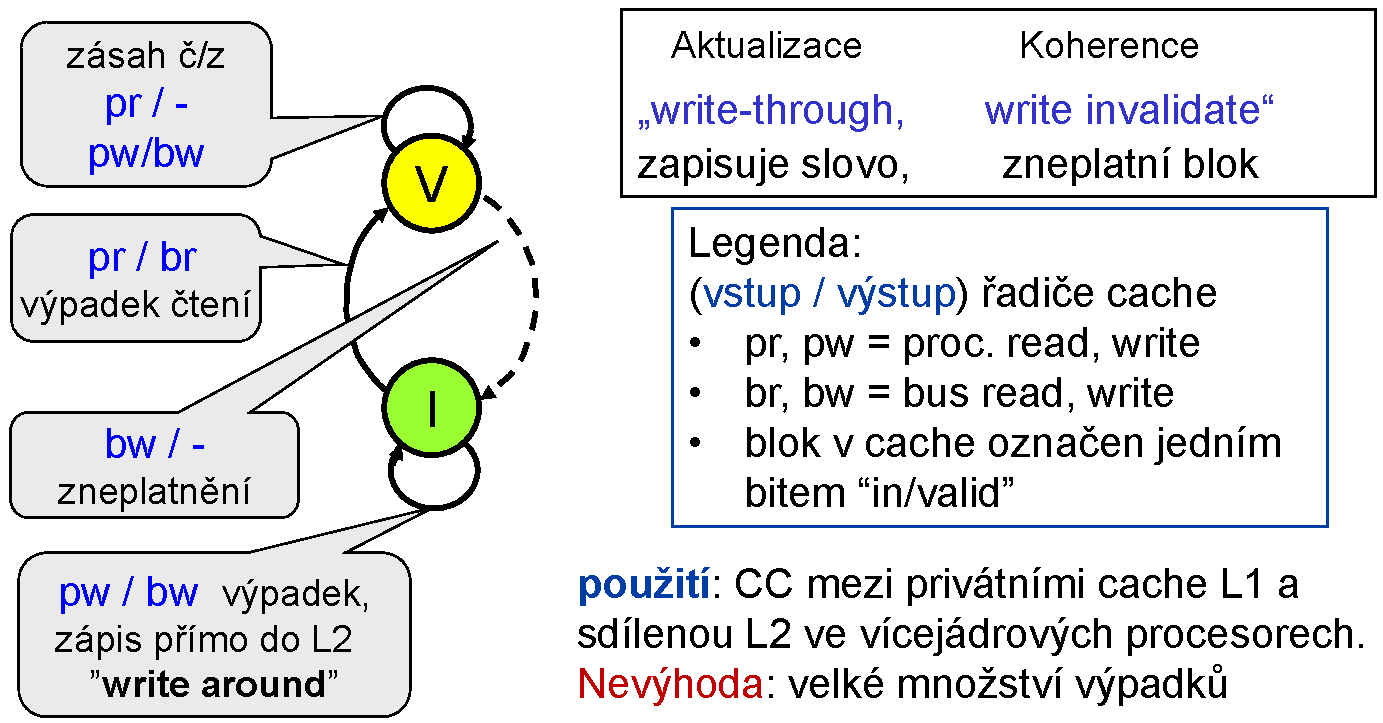
\includegraphics[width=0.9\linewidth]{dvoustavovy.pdf}
        \caption{Dvoustavový protokol na sběrnici. Plná čára -- co dělám já v lokální cache; čárkovaná -- co dělají cache jiných jader.}
    \end{figure}
\end{compactitem}

\subsection{Tří-stavový protokol MSI}

\begin{compactitem}
    \item Write-back, write-invalidate.
    \item Používá se všude jinde než mezi mezi L1 a L2.

    \item Aby se nemusely opakované zápisy do bloku cache neustále propisovat výš do SM, je možné špinavou kopii v L1 cache označit dalším stavem M a nechat ji v L1 co nejdéle (dokud nebude blok vybrán k výměně za jiný blok).

    \item Stavy bloku: \begin{compactitem}
        \item \textbf{Modifikovaný} (M, \textit{modified}) -- Jen 1 cache má platnou špinavou kopii, kopie ve sdílené paměti SM je zastaralá (dirty bit je 1).
        \item \textbf{Sdílený} (S, \textit{shared}) -- 1 nebo více pamětí cache má kopii shodnou se sdílenou pamětí SM (čistá kopie).
        \item \textbf{Neplatný} (I, \textit{invalid}) -- V této cache je pouze neplatná kopie (zastaralá).
    \end{compactitem}

    \item Blok S lze jen číst. Před zápisem musí CPU změnit jeho stav na M a
    ostatní kopie S musí být zneplatněny.

    \item CPU je pak jediný vlastník bloku M, má k němu exkluzivní přístup a
    může do něj zapisovat.

    \begin{figure}[H]
        \centering
        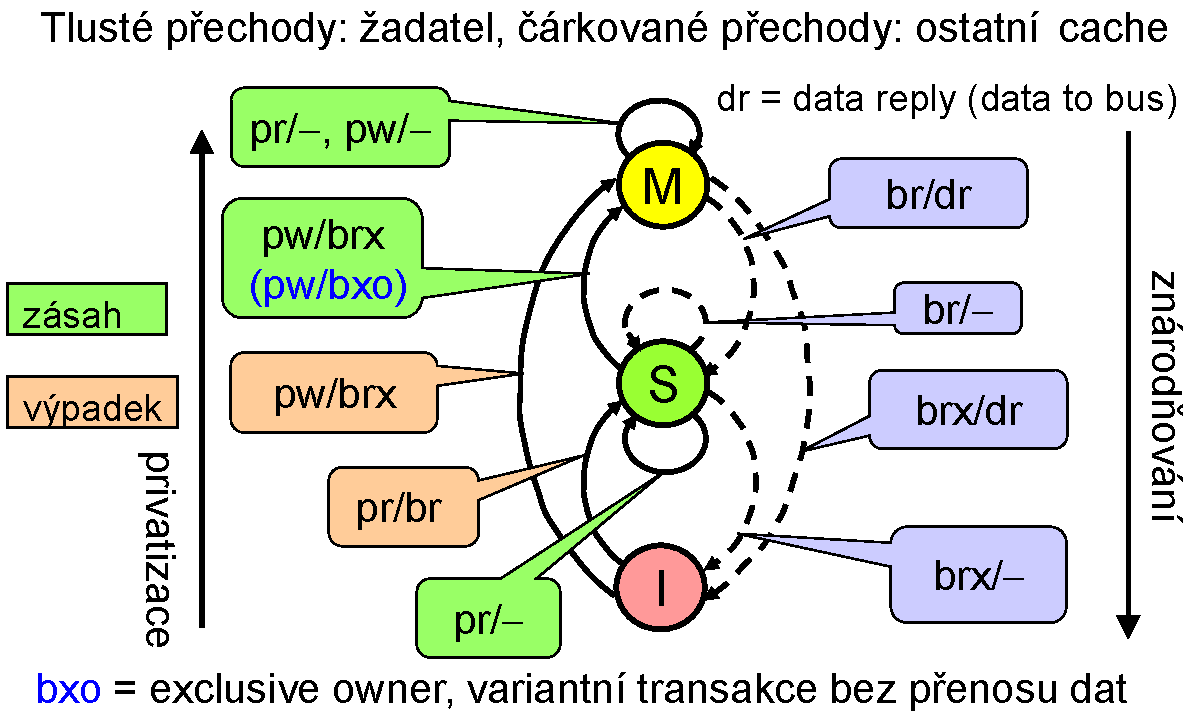
\includegraphics[width=0.9\linewidth]{msi.pdf}
        \caption{Třístavový protokol MSI.}
    \end{figure}
\end{compactitem}

\subsection{Čtyř-stavový protokol MESI}

\begin{figure}[H]
    \centering
    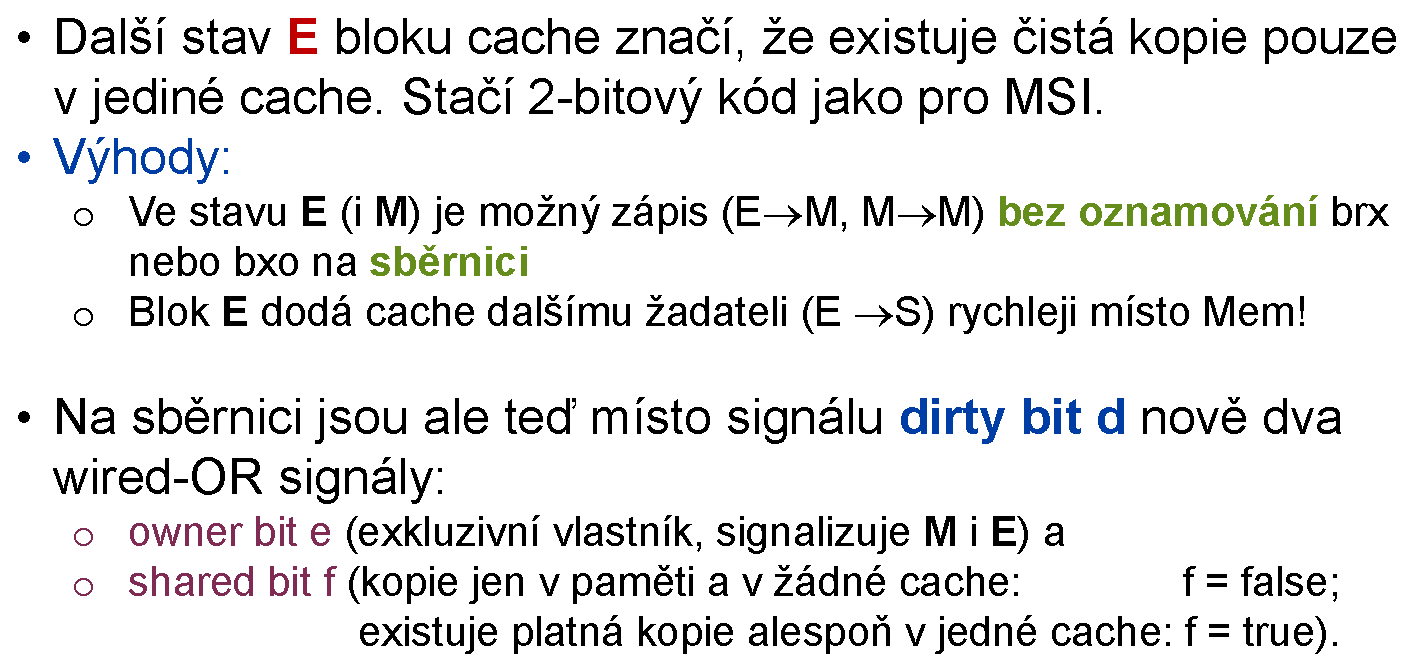
\includegraphics[width=0.9\linewidth]{mesi.pdf}
\end{figure}

\subsection{Pěti-stavový protokol MESIF}

\begin{compactitem}
    \item Intel
    \begin{figure}[H]
        \centering
        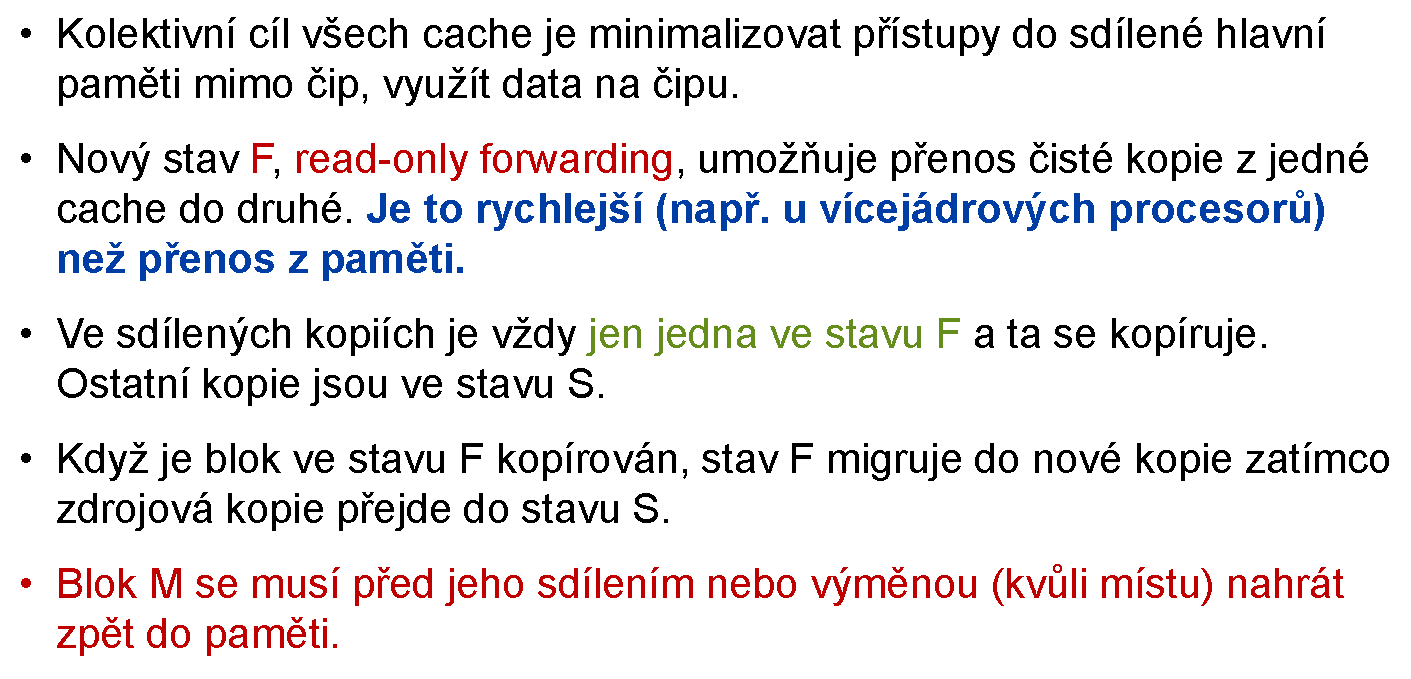
\includegraphics[width=0.9\linewidth]{mesif.pdf}
    \end{figure}
\end{compactitem}

\subsection{Pěti-stavový protokol MOESI}

\begin{compactitem}
    \item AMD
    \begin{figure}[H]
        \centering
        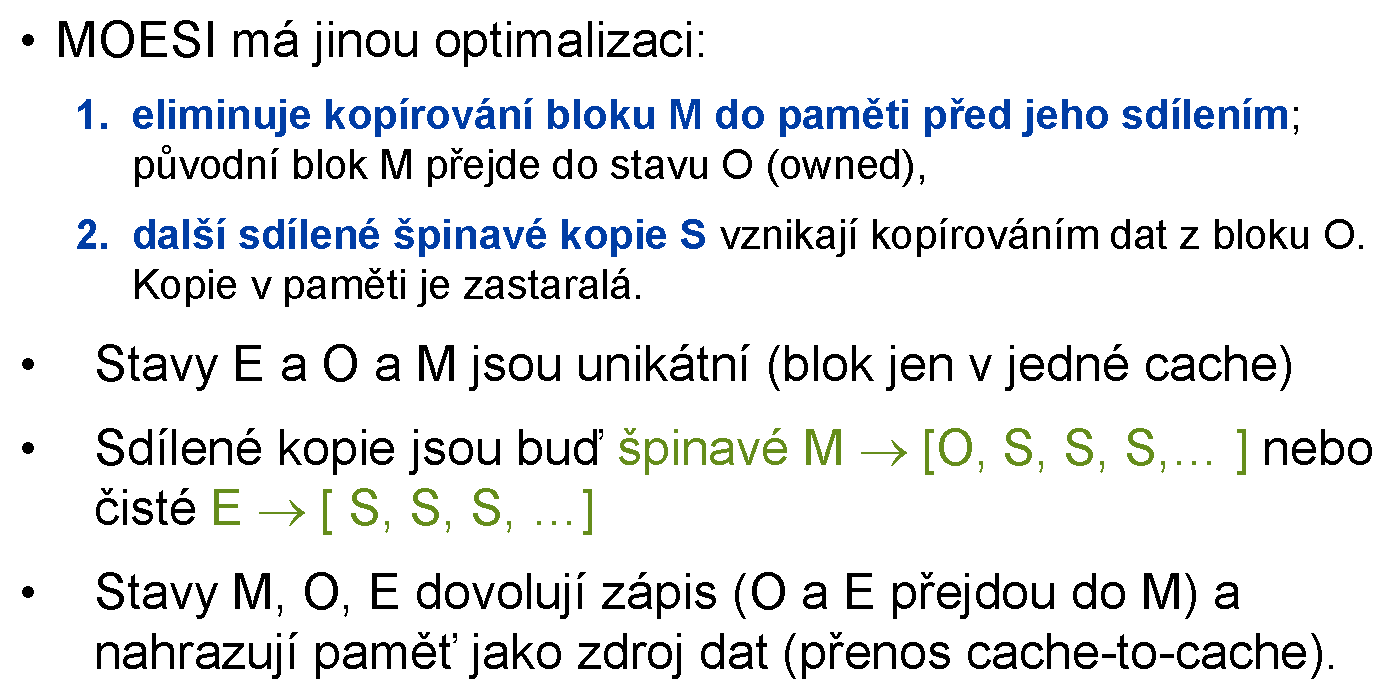
\includegraphics[width=0.9\linewidth]{moesi.pdf}
    \end{figure}
\end{compactitem}

%%%%%%%%%%%%%%%%%%%%%%%%%%%%%%%%%%%%%%%%%%%%%%%%%%%%%%%%%%%%%%%%%%%%%%%%%%%%%%%%

\section{Protokoly CC založené na distribuovaném adresáři}

\begin{compactitem}
    \item Stavy bloku paměti v jednotlivých cache jsou uloženy ještě odděleně v některém z adresářů. Žádost jde od žadatele přes domovský adresář bloku jen majitelům kopií, jen ti také odpovídají.

    \item Většinou používají NUMA systémy.

    \begin{figure}[H]
        \centering
        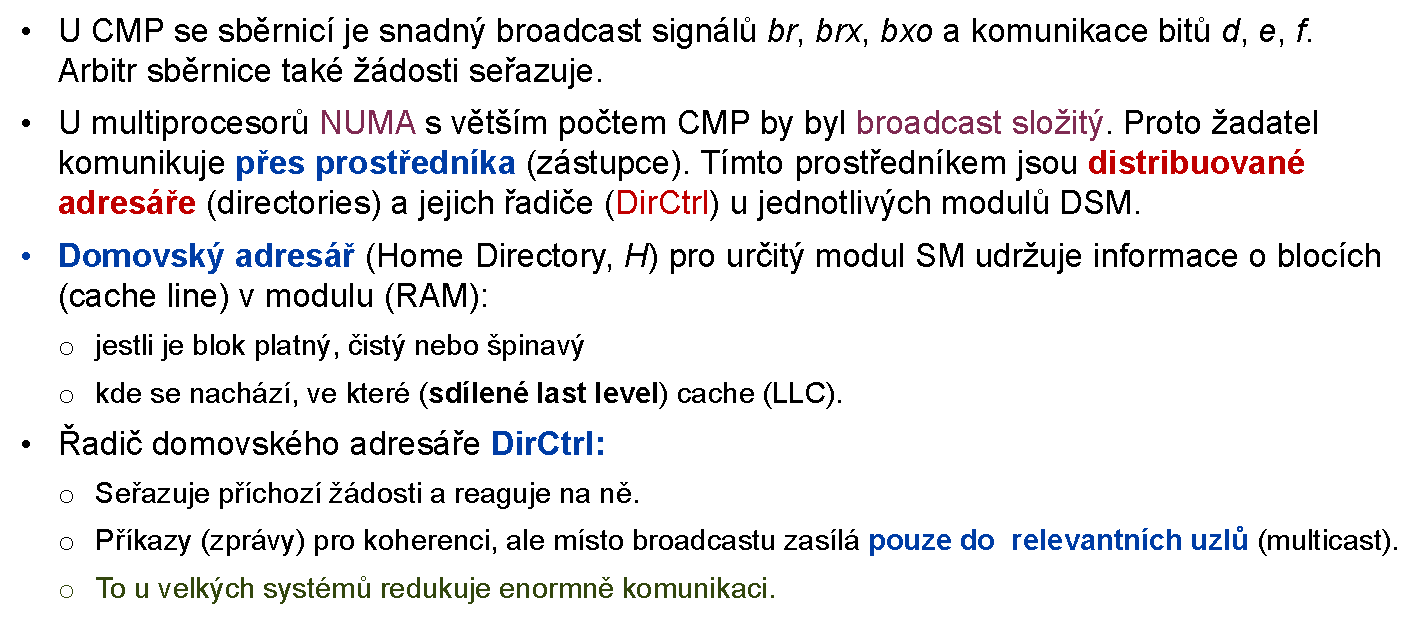
\includegraphics[width=1\linewidth]{distribuovane_1.pdf}
    \end{figure}

    \begin{figure}[H]
        \centering
        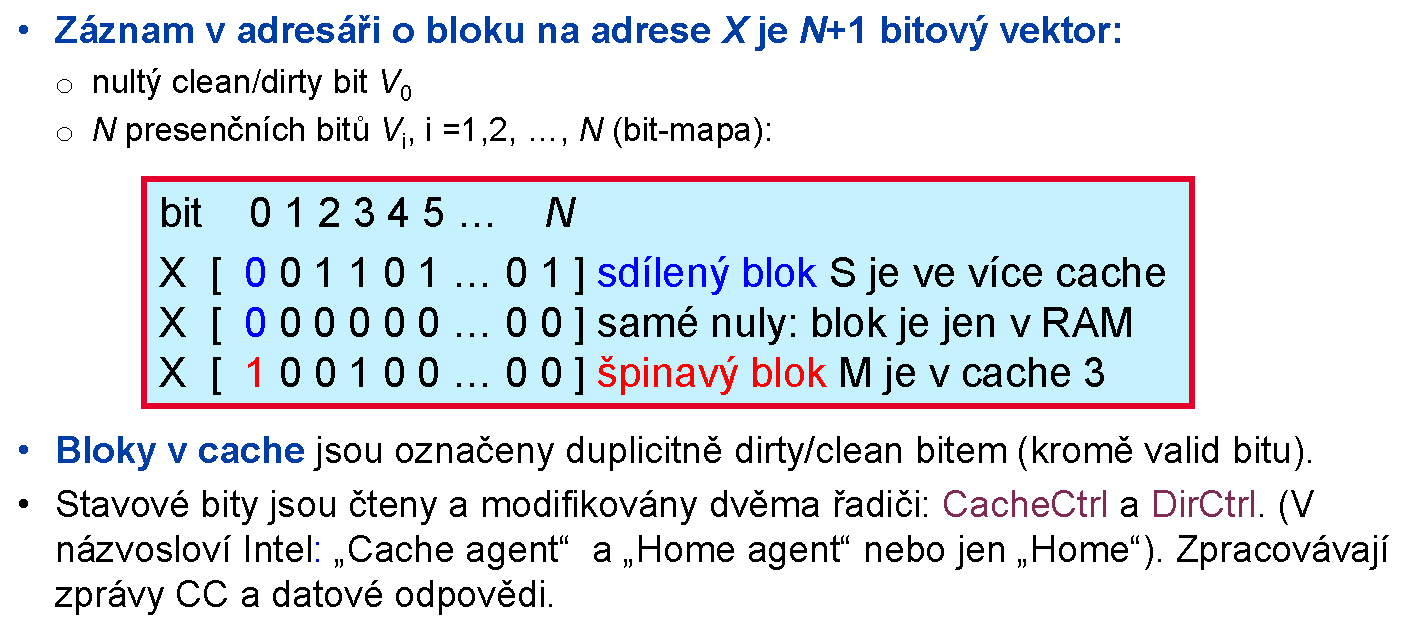
\includegraphics[width=1\linewidth]{distribuovane_2.pdf}
    \end{figure}

    \begin{figure}[H]
        \centering
        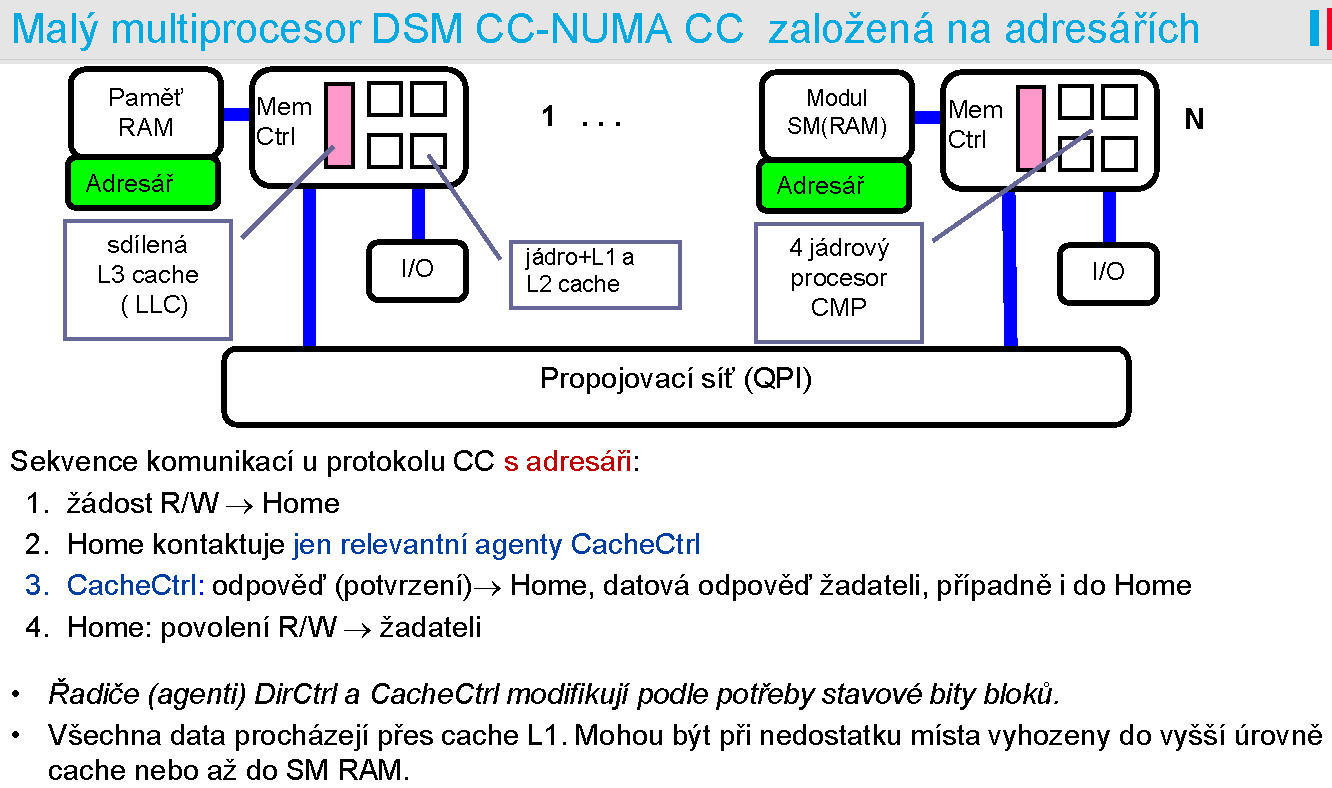
\includegraphics[width=1\linewidth]{distribuovane_3.pdf}
    \end{figure}
\end{compactitem}
